% !TeX root = ../main.tex
% 修改稿迁移版：自动编号，原文数据与待核事项保留。
\chapter{核心痛点与技术解决方案}
\section{命题约束与问题分析}\label{sec:3.1}
随着智能体从回答问题转向执行代码修复、功能开发等实际任务，企业需要为其提供能够运行程序、保存工作进度并隔离风险的执行环境。沙箱承担了这一职责，相当于为每个智能体配置一个独立的工作空间。随着智能体数量增加，如何在保障任务正常执行的同时控制资源投入，成为企业规模化部署必须解决的问题。

\subsection{命题约束}\label{sec:3.1.1}
华为提出的“高密部署智能体沙箱引擎”命题，将这一需求具体化：基于指定的 openEuler/\allowbreak{}Conch + StratoVirt 技术栈运行 OpenClaw，在管理面与容器总内存限制为 16GB、每个沙箱内部规格为 2U8G，即 2 个虚拟 CPU 和 8GB 内存、关闭 Swap 的条件下，提高能够同时运行并完成指定任务的智能体数量。命题要求在有限硬件内存中提高有效并发数，同时保证任务完成率和沙箱隔离。

\subsection{问题分析}\label{sec:3.1.2}
命题需要区分沙箱可见规格与宿主机实际物理内存占用。沙箱内部显示为 8GB 内存，实际运行过程中通常只使用其中一部分。单机可承载的智能体数量主要取决于单个沙箱的实际平均物理内存占用。PI OS 通过降低瞬时资源占用并根据任务阶段动态调度资源，提高高密部署能力。

\NumberedPara{1}{智能体的执行方式：大模型与工具交替进行}
智能体的资源使用特征由执行流程决定。智能体完成任务时，会在大模型（LLM）与三类工具之间交替调用：代码解释器（Code Sandbox）、无状态函数（Stateless Func）和有状态的 MCP Server 工具。以 TravelPlanner 为例，LLM 先生成计划，再调用工具查询交通信息、将计划写入同一 Notebook，最后执行筛选代码并形成出行方案。

\begin{figure}[H]\centering
\setcounter{figure}{0}

\includegraphics[width=.95\linewidth,height=.50\textheight,keepaspectratio]{figures/updated-3-1.png}
\caption{智能体任务中 LLM 与工具的交替调用流程}\label{fig:3-1}
\end{figure}
图示表明，LLM 推理与工具执行呈交替关系。LLM 推理期间工具暂停计算，工具执行期间 LLM 等待结果。工具在等待阶段仍保留运行状态，由此产生持续的内存占用。

\begin{enumerate}
\item 三类工具的需求彼此异构
\end{enumerate}
不同智能体任务需要保留的状态完全不同。下面是项目测试中六类典型 Agent 负载的资源画像，差异极大：

\begin{figure}[H]\centering
\setcounter{figure}{1}
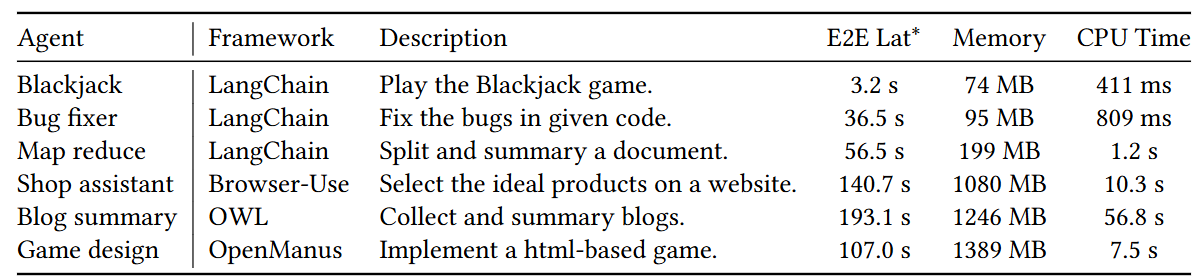
\includegraphics[width=.95\linewidth,height=.32\textheight,keepaspectratio]{figures/image9.png}
\par{\fontsize{9}{12}\selectfont (a) 原始观测与项目架构}\par\vspace{5pt}
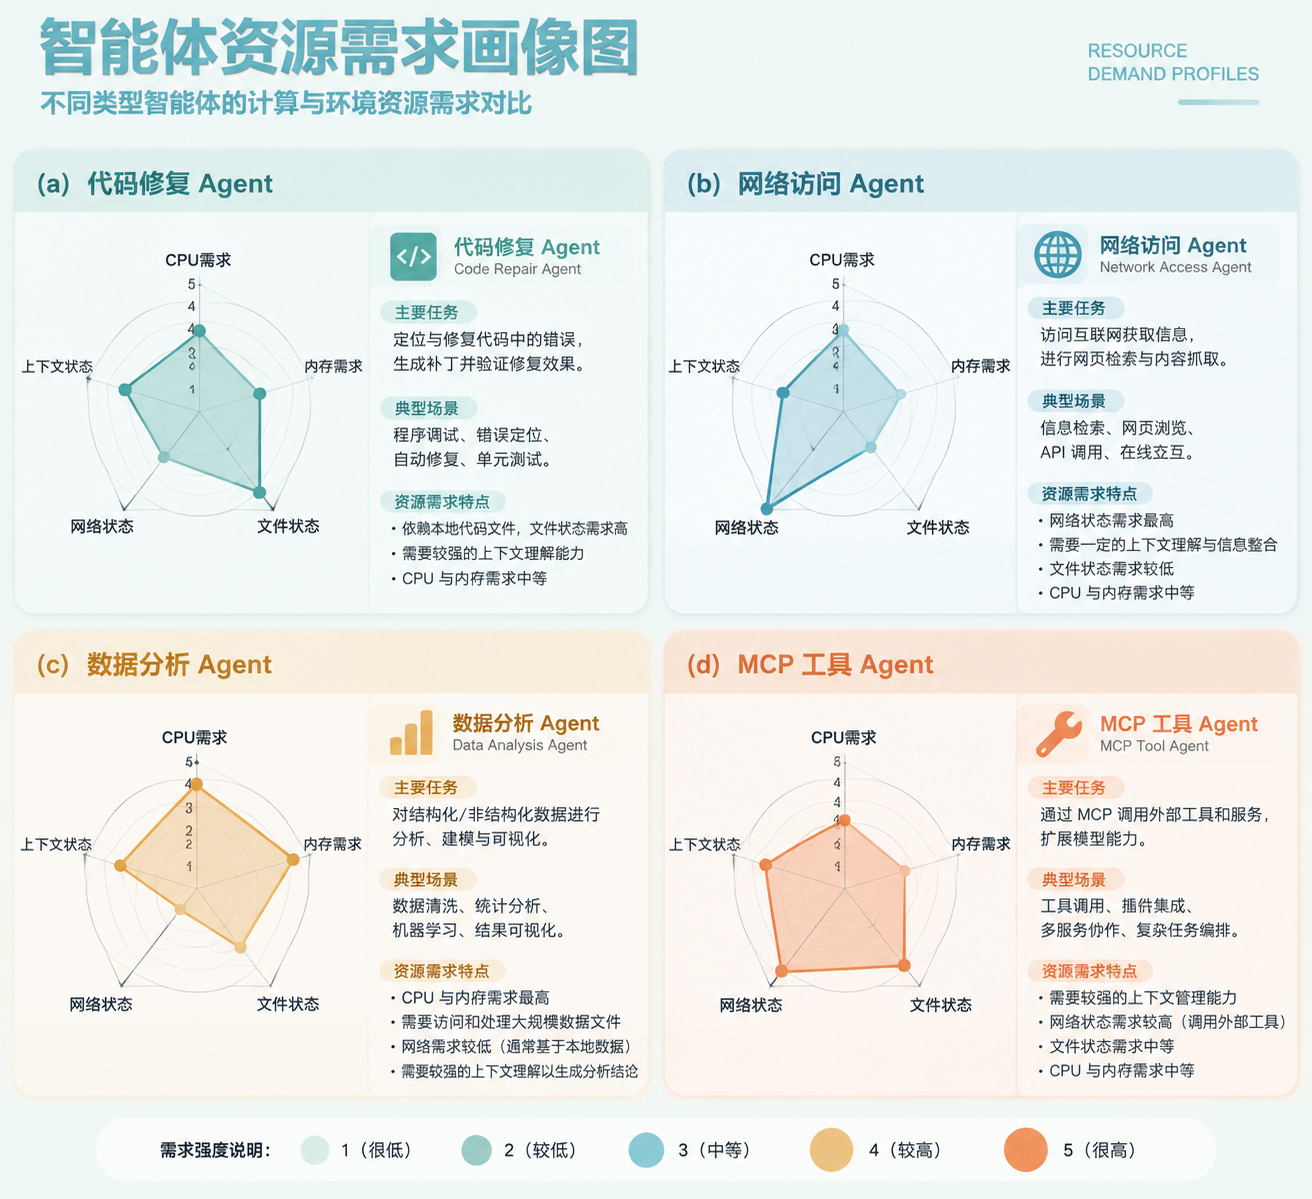
\includegraphics[width=.95\linewidth,height=.40\textheight,keepaspectratio]{figures/updated-3-2.png}
\par{\fontsize{9}{12}\selectfont (b) 资源需求与系统分层概览}\par
\caption{典型智能体任务的资源画像}\label{fig:3-2}
\par\vspace{3pt}{\fontsize{9}{12}\selectfont\linespread{1}\selectfont 注：(a) 为六类典型负载的原始资源观测；(b) 为所供图稿中的四类资源需求示意，不表示实测数值，不替代原始观测。}
\end{figure}
以代码修复任务为例，ls、cat、sed 等命令通常在毫秒级完成，主要使用文件系统和少量内存；wget 等外网访问命令需要网络能力；数据分析程序需要保留较大的内存对象；有状态 MCP 工具需要保留发生变化的内存和寄存器状态。不同工具具有分层、异构的资源需求，现有运行时通常对完整环境进行统一保存和恢复，由此产生额外开销。

项目据此将部署密度问题划分为运行时冗余、资源空转和状态重复三个相互关联的方面，并分别提出对应方案。

\section{问题 1：运行时冗余}\label{sec:3.2}
运行时冗余，是指沙箱为了执行具体任务，需要额外维持一套较重的系统环境，而其中相当一部分功能并未被当前任务实际使用。

以代码修复为例，智能体主要执行项目文件读取、代码编辑、测试和结果保存，核心资源是文件系统与少量内存。通用执行环境还会维护后台服务、管理组件和其他系统功能，其中部分组件与当前任务无直接关系，却持续占用内存并增加初始化和状态管理开销。

通用运行组件在每个沙箱中重复加载，固定开销会随实例数量增长，压缩可用于任务执行的内存空间。图 3-3 展示单实例在启动和运行阶段的内存构成：Runtime（沙箱运行环境）和 Sandbox（沙箱开销）构成每个实例的固定成本，Waste 表示资源争用或过度配置产生的额外占用。

\begin{figure}[H]\centering
\setcounter{figure}{2}
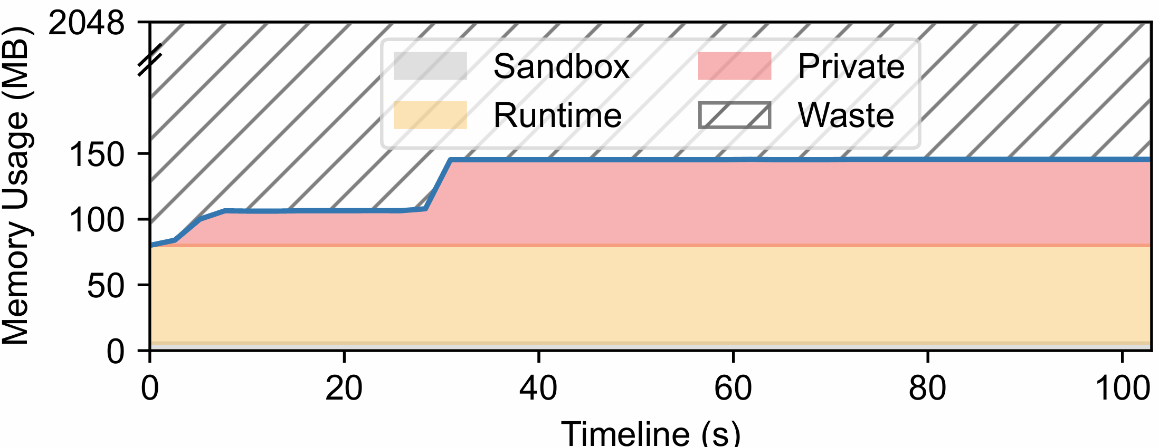
\includegraphics[width=.95\linewidth,height=.50\textheight,keepaspectratio]{figures/image10.png}
\caption{单实例运行过程中的内存构成}\label{fig:3-3}
\end{figure}
冗余的根源有三层：

\begin{enumerate}
\item Linux 快照与恢复粒度较粗：CRIU（Checkpoint and Restore in Userspace）通常对沙箱整体状态进行保存，保存和恢复的数据量较大。
\item Linux 页置换机制（kswapd）采用通用的被动回收策略，缺少智能体任务语义，可能置换活跃页或遗漏闲置资源。
\item 网络协议栈状态的恢复成本较高：TCP/\allowbreak{}UDP 连接、Socket 和网络命名空间的恢复需要频繁调用内核并竞争锁，耗时通常高于普通内存页恢复。
\end{enumerate}
\section{解决方案 1：运行时扁平化}\label{sec:3.3}
运行时扁平化将每个智能体的完整运行环境拆分为“轻量运行库 + 系统级共享服务”。系统据此识别工具依赖、状态位置和当前执行所需功能，减少每个沙箱的固定开销。

\begin{enumerate}
\item LibOS（Guest Kernel，用户态内核）：在用户态实现文件系统、网络和内存管理等应用所需功能，减少对宿主内核共享路径的依赖和锁竞争，降低运行开销。
\item 系统服务（Services）：将网络协议栈、文件系统等通用能力从沙箱内部抽离，形成多实例共享服务。沙箱保留任务相关状态，并在访问外网、大模型或文件时按需建立对应的隔离上下文和数据通路，从而降低完整系统组件的重复部署开销。
\end{enumerate}
PI OS 系统架构

\begin{figure}[H]\centering
\setcounter{figure}{3}
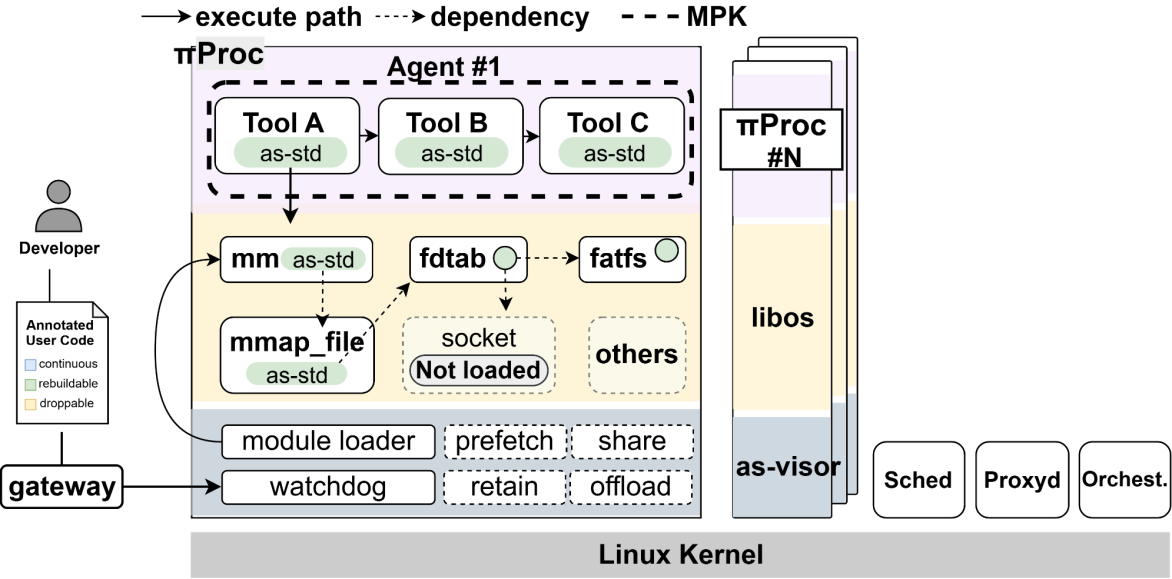
\includegraphics[width=.95\linewidth,height=.25\textheight,keepaspectratio]{figures/image11.png}
\par{\fontsize{9}{12}\selectfont (a) 原始观测与项目架构}\par\vspace{5pt}
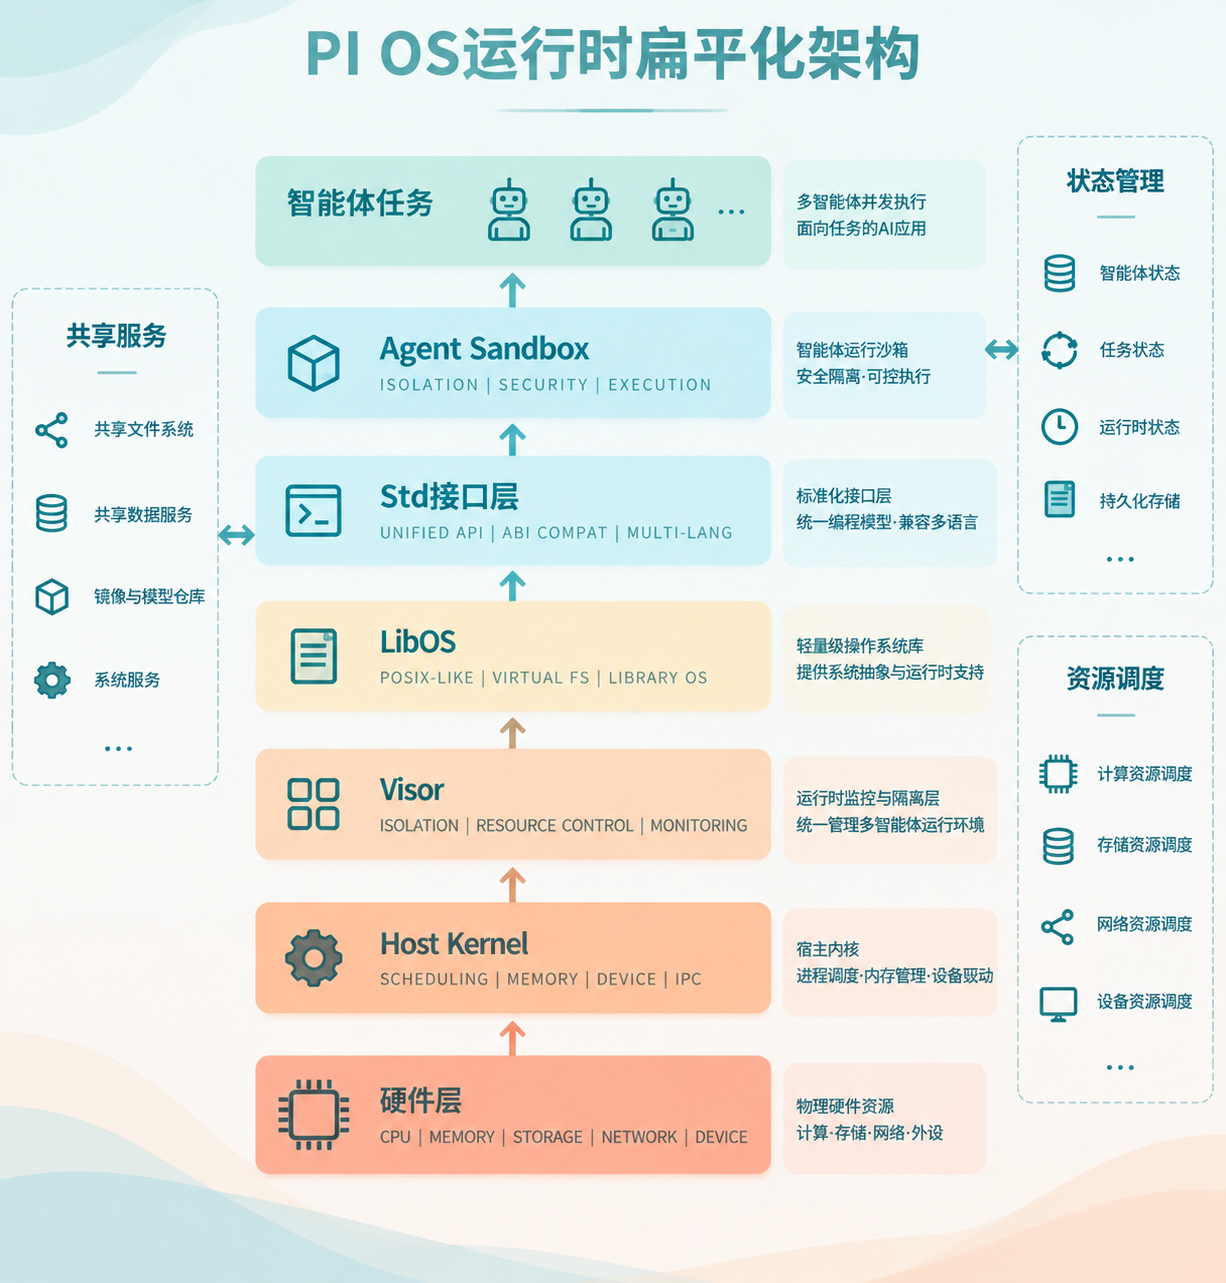
\includegraphics[width=.95\linewidth,height=.42\textheight,keepaspectratio]{figures/updated-3-4.png}
\par{\fontsize{9}{12}\selectfont (b) 资源需求与系统分层概览}\par
\caption{PI OS 运行时扁平化系统架构}\label{fig:3-4}
\par\vspace{3pt}{\fontsize{9}{12}\selectfont\linespread{1}\selectfont 注：(a) 为项目组件职责架构；(b) 为所供图稿的分层概览，组件协同与边界以本节说明为准。}
\end{figure}
扁平化架构包含四个关键角色：

\begin{enumerate}
\item Std 接口：识别 Tool 启动依赖，确定卸载和恢复所需状态，按状态类型分配内存，作为统一运行时抽象层的语义入口；
\item LibOS：用户态 Guest Kernel，承接文件系统、网络和内存管理等功能，作为精简后的运行内核；
\item Visor：与集群调度器、LLM Proxy 和 Kernel 状态池交互，执行卸载与预取，负责沙箱与宿主机之间的状态传输和协调；
\item Sched /\allowbreak{} Proxyd /\allowbreak{} Orchest：管理全局卸载、加载和预取任务，并结合修改后的 Linux 内核完成资源管理和集群侧调度。
\end{enumerate}
\section{问题 2：资源空转}\label{sec:3.4}
资源空转，是指工具暂时停止计算后，其运行环境和任务状态仍持续占用资源，其他智能体无法充分利用这部分容量。

智能体按照“LLM 分析与决策、工具执行、结果返回”的顺序循环运行。代码修复任务完成一次测试后，工具会等待 LLM 分析报错并生成下一步指令。等待期间 CPU 计算停止，内存对象和运行上下文仍保持驻留。销毁环境会中断任务状态，完整快照则会增加额外的数据搬运。

图 3-5 记录项目测试中的单实例 CPU 与内存使用时序：计算集中在 init、step1 等短时窗口，CPU 峰值为 209.7\%；其余时间 CPU 接近 0，内存仍维持在 447.7MB 附近，显示等待阶段存在明显的内存驻留。

\begin{figure}[H]\centering
\setcounter{figure}{4}
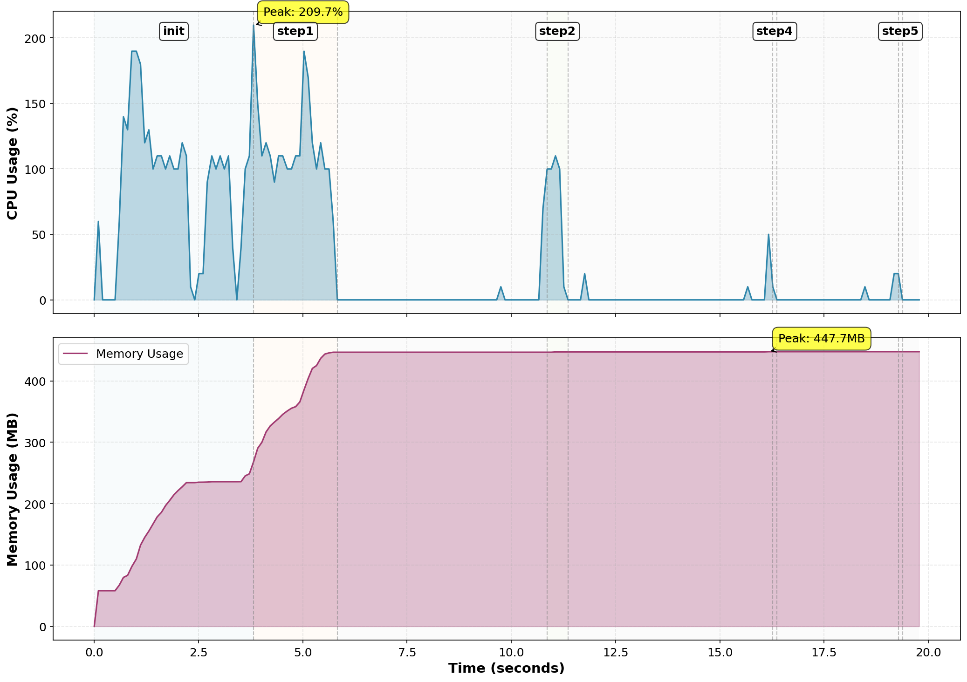
\includegraphics[width=.95\linewidth,height=.50\textheight,keepaspectratio]{figures/image12.png}
\caption{单实例 CPU 与内存使用时序}\label{fig:3-5}
\end{figure}
空转体现在两个维度：

\NumberedPara{1}{工具执行阶段（空间维度）：不同工具具有异构执行需求，统一资源配置会产生分配冗余；}
\NumberedPara{2}{LLM 推理阶段（时间维度）：主流方案为保证数据安全和任务连续性，通常保留沙箱全部运行状态，等待期间形成资源闲置。}
\section{解决方案 2：动态资源卸载}\label{sec:3.5}
动态资源卸载利用智能体执行阶段信息，在工具暂停计算时释放可回收资源，并根据下一次调用的实际需求恢复状态。PI OS 在关闭操作系统 Swap 的条件下显式管理运行状态。该机制由分层状态卸载与按需状态恢复两个子任务协同完成。

\subsection{分层状态卸载：按状态类型实施保留与恢复}\label{sec:3.5.1}
该机制将运行时状态划分为文件、网络、内存、CPU 和寄存器等类型，并分别设置保留与恢复策略，实现闲置资源及时回收。具体包括三个方面：

\begin{enumerate}
\item 构建统一运行时抽象层，识别 Agent 状态的类型、用途和生命周期；
\item 在沙箱接口层完成状态分类与管理，并扩展 Python 运行时，支持对文件、网络、内存、CPU 和寄存器状态分别捕获与卸载；
\item 扩展 Linux 内核系统服务与沙箱协同机制，依据状态语义分配资源，降低活跃状态被错误置换的概率。
\end{enumerate}
为支撑该机制，内核侧新增卸载、预加载、激活和释放接口，由系统根据状态语义触发。以 struct agent\_park\_task 为例，retain\_bytes、durable\_bytes 和 durable\_extents[] 分别记录保留状态量、持久化状态量与持久化区间，io\_budget 记录字节数、预计耗时和松弛时间，为内核提供可执行的卸载约束。

\subsection{按需状态恢复：由状态访问触发加载}\label{sec:3.5.2}
每轮执行通常只涉及部分系统功能。按需恢复机制在状态被访问时加载对应组件，降低全量恢复产生的冷启动开销：

\begin{enumerate}
\item 语义截获与转发：对运行时组件修改，截获执行中对文件/\allowbreak{}网络/\allowbreak{}内存的访问请求；
\item 恢复流程组装引擎：访问缺失时，按捕获的请求动态组装恢复流程（如仅恢复文件句柄、重建网络连接、加载内存快照），实现按需加载与重建；
\item 细粒度组件索引：为每个状态组件（单个文件、网络连接、内存区域）解耦，支持快速定位、独立恢复。
\end{enumerate}
\begin{figure}[H]\centering
\setcounter{figure}{5}
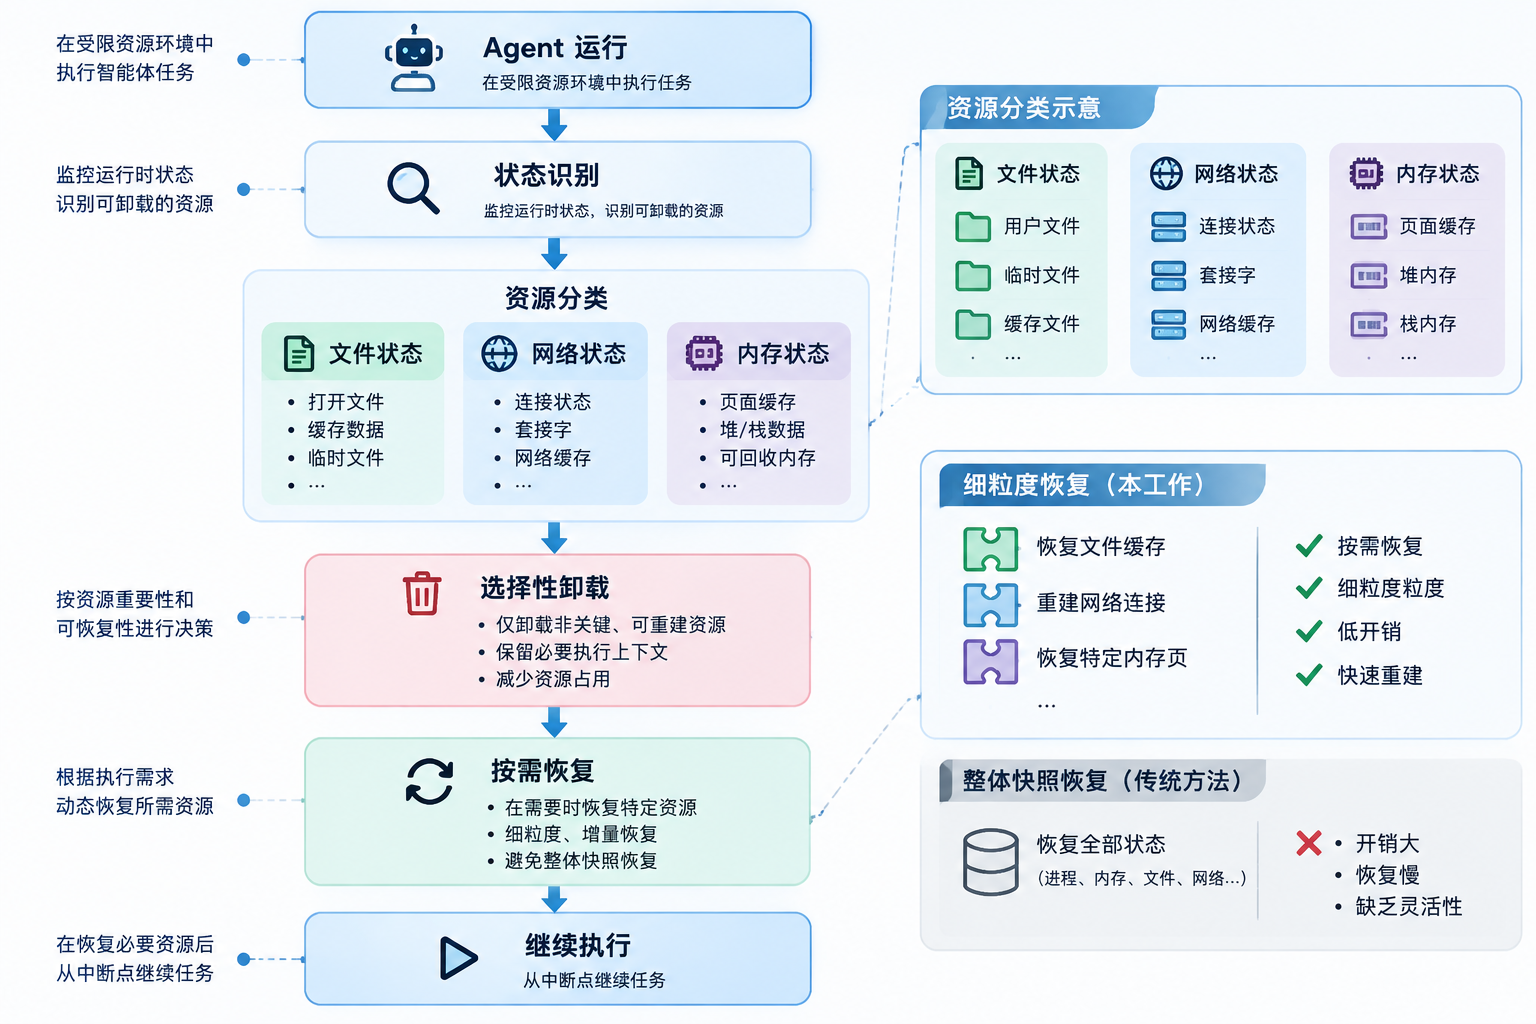
\includegraphics[width=.95\linewidth,height=.50\textheight,keepaspectratio]{figures/updated-3-6.png}
\caption{PI OS 动态资源卸载与恢复流程}\label{fig:3-6}
\end{figure}
\subsection{语义感知的实现路径}\label{sec:3.5.3}
\NumberedPara{1}{运行时触发（主路径）：在 Guest Kernel 系统库中设置资源访问触发点。wget 调用触发网络挂载，目录操作触发文件系统恢复。资源访问事件直接提供所需状态类型，提高识别精度。}
\NumberedPara{2}{规则感知与预取（可选增强）：在大模型输出 Token 流时解析 tool call 字段，识别下一步调用并预取所需状态。预取阶段仅加载相关状态，业务操作仍由正式工具调用触发；调用信息不足时，系统转由实际状态访问事件触发恢复。}
\subsection{实测效果}\label{sec:3.5.4}
端到端：测试中，PI OS（启用语义卸载）在约\textbf{0.7 秒}额外延迟下，将总内存用量降低\textbf{78.5\%}--\textbf{91.7\%}；完整沙箱全量快照与恢复（Full CR）产生约\textbf{6.0 秒}延迟，内存用量降低\textbf{25\%}。

\begin{figure}[H]\centering
\setcounter{figure}{6}
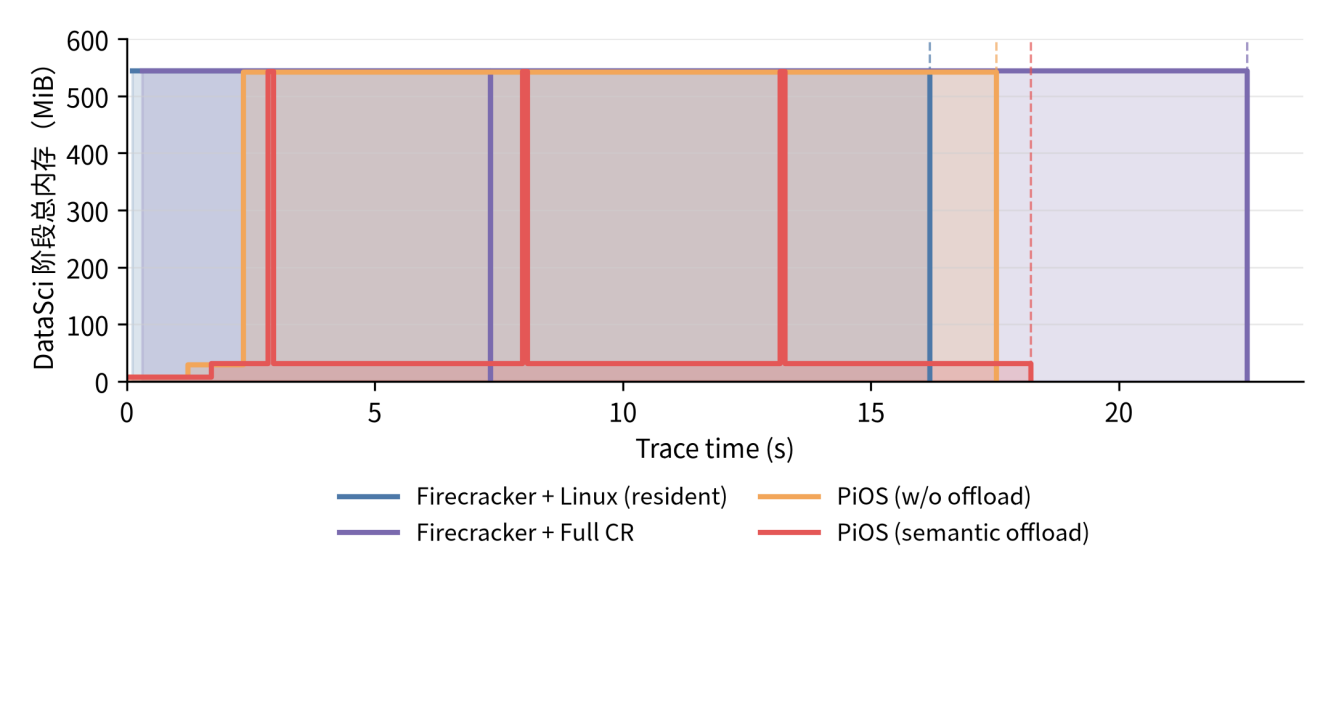
\includegraphics[width=.95\linewidth,height=.29\textheight,keepaspectratio]{figures/image14.png}
\par{\fontsize{9}{12}\selectfont (a)}\par\vspace{4pt}
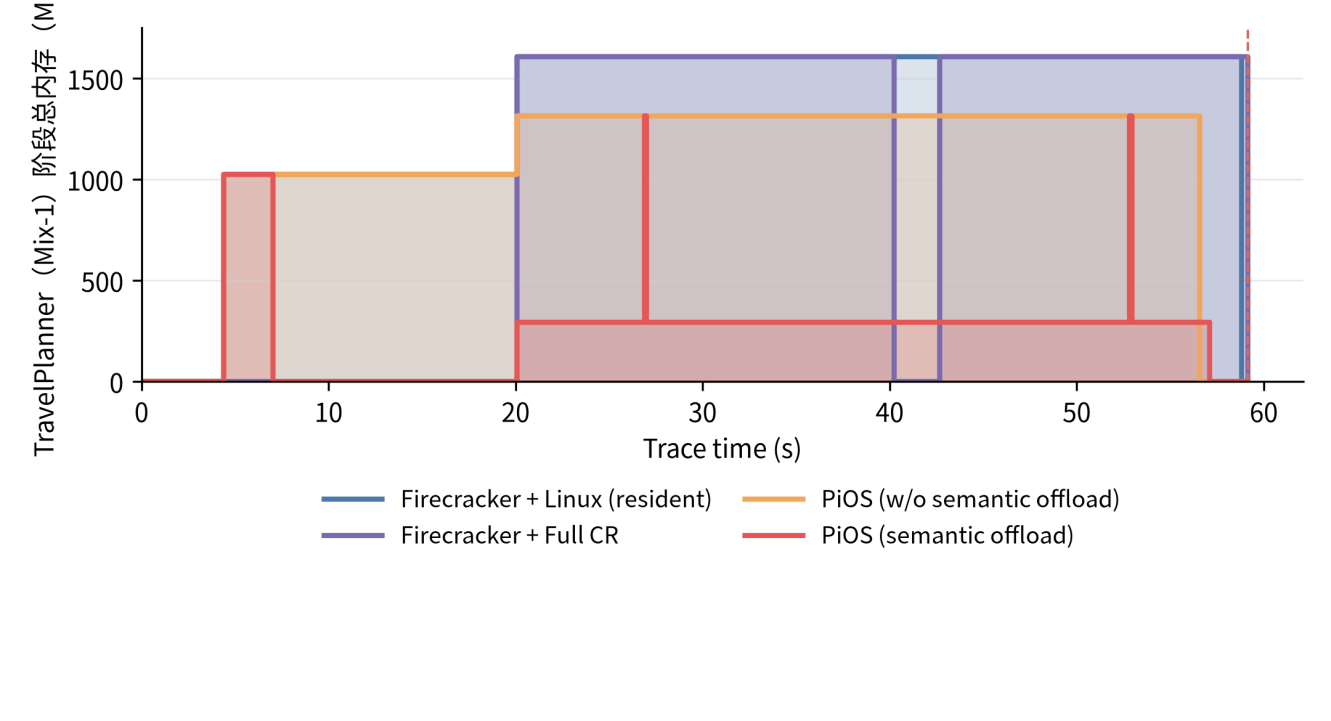
\includegraphics[width=.95\linewidth,height=.29\textheight,keepaspectratio]{figures/image15.png}
\par{\fontsize{9}{12}\selectfont (b)}\par\vspace{4pt}
\caption{不同数据集下的内存占用对比}\label{fig:3-7}
\end{figure}
\FloatBarrier
\begingroup\linespread{1}\selectfont
\setcounter{table}{0}
\begin{longtable}{@{}>{\raggedright\arraybackslash}p{\dimexpr 0.24841\linewidth-1.4904\tabcolsep\relax}>{\raggedright\arraybackslash}p{\dimexpr 0.21141\linewidth-1.2684\tabcolsep\relax}>{\raggedright\arraybackslash}p{\dimexpr 0.21141\linewidth-1.2684\tabcolsep\relax}>{\raggedright\arraybackslash}p{\dimexpr 0.32878\linewidth-1.9727\tabcolsep\relax}@{}}
\caption{卸载开销对比（5 次取中位数）}\label{tab:3-1}\\
\hline
\rowcolor{WordTableHeader} \TableHeaderText{Benchmark} & \TableHeaderText{Full CR 卸载} & \TableHeaderText{PI OS 卸载} & \TableHeaderText{结果说明} \\ \hline
\endfirsthead
\multicolumn{4}{c}{\fontsize{9}{12}\selectfont 表 3-1（续）}\\
\hline
\rowcolor{WordTableHeader} \TableHeaderText{Benchmark} & \TableHeaderText{Full CR 卸载} & \TableHeaderText{PI OS 卸载} & \TableHeaderText{结果说明} \\ \hline
\endhead
\hline\endfoot\hline\endlastfoot
\rowcolor{WordTableStripe} 
DataSci & 7,763.6 ms & 118.261 ms & PI OS 加速 64.6 倍 \\ \hline
TravelPlanner & 7,836.4 ms & 16.38 ms & PI OS 共享部分驻留内存 \\ \hline
\end{longtable}\endgroup
冷启动：单个沙箱约\textbf{1.3 ms}完成冷启动，启动时间减少\textbf{92.5\%}。Full CR 在未预取情况下通过缺页异常加载内存，增加约\textbf{6.0 秒}；加入预取后，额外时间约为\textbf{0.7 秒}。

受限资源下的系统级对比（Resident 状态常驻 vs Compact 紧凑模式）：在\textbf{8GB}内存、\textbf{4}CPU 上限、\textbf{6 秒}错峰拉起、DataSci 负载下，两组均完成全部\textbf{48}个任务、\textbf{0}次 OOM：

\FloatBarrier
\begingroup\linespread{1}\selectfont
\setcounter{table}{1}
\begin{table}[H]\centering
\caption{受限资源下的系统级性能对比}\label{tab:3-2}
\color{TableText}\fontsize{9pt}{12.6pt}\selectfont
\begin{tabular}{@{}>{\raggedright\arraybackslash}p{\dimexpr 0.40984\linewidth-2.4590\tabcolsep\relax}>{\raggedright\arraybackslash}p{\dimexpr 0.19672\linewidth-1.1803\tabcolsep\relax}>{\raggedright\arraybackslash}p{\dimexpr 0.19672\linewidth-1.1803\tabcolsep\relax}>{\raggedright\arraybackslash}p{\dimexpr 0.19672\linewidth-1.1803\tabcolsep\relax}@{}}
\hline
\rowcolor{WordTableHeader} \TableHeaderText{指标} & \TableHeaderText{Resident} & \TableHeaderText{Compact} & \TableHeaderText{提升/\allowbreak{}变化} \\ \hline
\rowcolor{WordTableStripe} 
QEMU 宿主机平均 CPU（\%CPU） & 229.7\% & 465.0\% & 2.02\ensuremath{\times}（+102.5\%） \\ \hline
Guest RSS 峰值（GiB） & 7.59 GiB & 7.79 GiB & +0.20 GiB（+2.68\%） \\ \hline
\rowcolor{WordTableStripe} 
系统吞吐量（batch/\allowbreak{}s） & 0.007072 & 0.021236 & 3.003\ensuremath{\times}（+200.3\%） \\ \hline
已验证安全并发（个） & 8 & \ensuremath{\geq}48 & \ensuremath{\geq}6\ensuremath{\times} \\ \hline
\end{tabular}
\end{table}\endgroup
\section{问题 3：状态重复}\label{sec:3.6}
状态重复，指多个沙箱或同一任务的不同执行轮次，分别保存了内容相同、本可安全复用的状态。

Agent 运行时通常基于隔离的执行环境构建，每个实例独立加载和存储所需状态。于是：

\begin{enumerate}
\item 相同的高频复用状态（预训练模型权重、代码依赖库、数据集、配置文件）在不同实例间被重复存储；
\item 现有 mmap 等文件级共享机制受执行环境隔离和检查点恢复影响，相同状态在不同实例间仍以独立副本存在，形成重复占用。
\end{enumerate}
\begin{figure}[H]\centering
\setcounter{figure}{7}
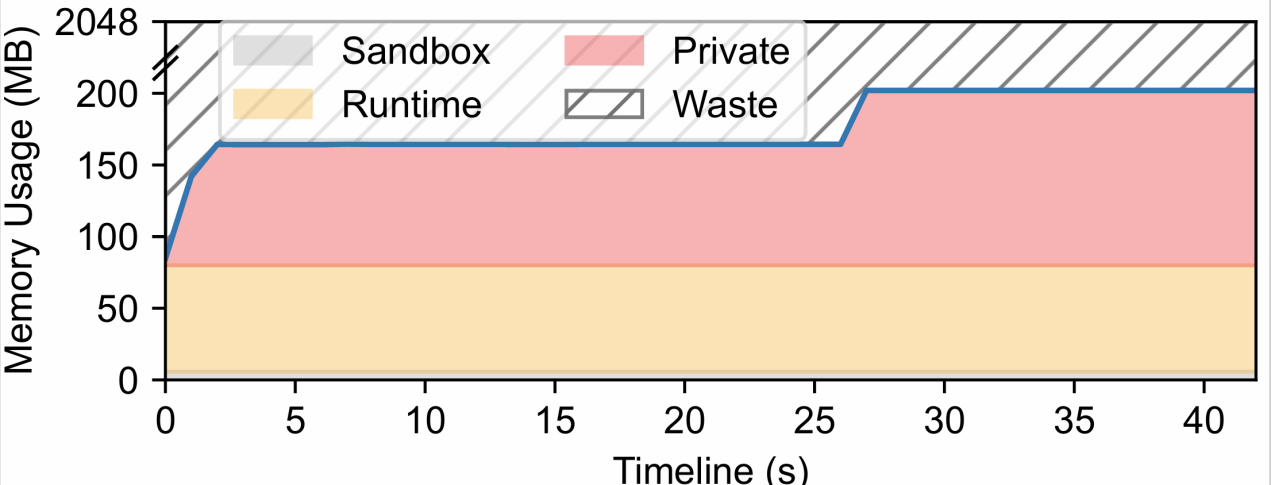
\includegraphics[width=.95\linewidth,height=.50\textheight,keepaspectratio]{figures/image16.png}
\caption{传统沙箱实例中的重复状态占用}\label{fig:3-8}
\end{figure}
三个技术挑战：

\begin{enumerate}
\item 副本冗余：在隔离环境中如何识别并消除相同状态的重复存储？
\item 共享语义丢失：在状态检查点与恢复过程中如何维持共享语义，避免状态分裂？
\item 共享粒度粗：如何设计细粒度、语义感知的共享机制，匹配智能体多样化的状态类型？
\end{enumerate}
共享边界由内容、版本、访问权限和状态可变性共同确定。任务凭据、私人文件、会话状态和可修改中间结果保留独立副本，以满足隔离和一致性要求。

\section{解决方案 3：智能内存共享}\label{sec:3.7}
智能内存共享通过为状态添加语义标识并构建共享状态池，实现跨实例去重以及文件和网络状态复用。系统根据状态用途、生命周期、版本和访问权限确定共享范围，并为私有或可修改状态保留独立副本。

三个层面：

\begin{enumerate}
\item 多级状态管理机制：为不同类型智能体运行时提供多级状态标识，支持跨智能体、跨实例、跨阶段的多级共享。
\item 系统级共享文件/\allowbreak{}网络服务：在保证安全的条件下，构建用户态与系统态协同的共享池，支持文件、网络的调用共享，提高资源使用与读写吞吐。
\item 共享语义维持机制：在状态检查点与恢复过程中，用“引用计数 + 写时复制（Copy-on-Write）”维持共享语义，避免状态分裂，确保共享状态一致。
\end{enumerate}
工程落地细节：

\begin{enumerate}
\item 语义识别在运行时侧完成：cat、sed 等命令触发文件系统相关操作，进而按需恢复文件系统；curl 触发网络相关操作；Python 内部通过修改 Python 运行时，在具体语句执行发现状态缺失时按需加载。
\item 预取机制在大模型输出 Token 时解析下一步工具调用并提前加载相关状态，以适应执行路径的动态变化。
\item 共享判断的边界：应同时考虑内容、版本与访问权限。同版本只读依赖文件可作为共享候选；不同任务各自修改的文件、用户凭据、会话数据应保留私有副本；内容相同也不必然允许跨租户共享，需按安全策略限制共享范围。
\item 范围限定：现阶段支持 Python 与 Bash，多语言支持将在后续版本中扩展。
\end{enumerate}
\FloatBarrier
\begingroup\linespread{1}\selectfont
\setcounter{table}{2}
\begin{longtable}{@{}>{\raggedright\arraybackslash}p{\dimexpr 0.42148\linewidth-0.8430\tabcolsep\relax}>{\raggedright\arraybackslash}p{\dimexpr 0.57852\linewidth-1.1570\tabcolsep\relax}@{}}
\caption{PI OS 关键成果指标}\label{tab:3-3}\\
\hline
\rowcolor{WordTableHeader} \TableHeaderText{指标} & \TableHeaderText{目标值} \\ \hline
\endfirsthead
\multicolumn{2}{c}{\fontsize{9}{12}\selectfont 表 3-3（续）}\\
\hline
\rowcolor{WordTableHeader} \TableHeaderText{指标} & \TableHeaderText{目标值} \\ \hline
\endhead
\hline\endfoot\hline\endlastfoot
\rowcolor{WordTableStripe} 
内存占用减少 & \ensuremath{\geq}30\% \\ \hline
系统整体吞吐量提升 & \ensuremath{\geq}25\% \\ \hline
\rowcolor{WordTableStripe} 
跨实例去重 & 模型权重 /\allowbreak{} 依赖库等高复用状态去重 \\ \hline
\end{longtable}\endgroup
三项方案形成连续的技术路径：运行时扁平化降低基础环境开销并提供状态管理接口；动态资源卸载回收任务等待阶段的闲置资源；智能内存共享消除多个实例间的重复状态。三项方案分别优化固定运行开销、等待阶段驻留开销和跨实例重复占用。

企业部署价值通过规定内存预算下的有效沙箱并发数、任务成功率、完成时间和单任务资源成本进行评估。项目将在相同硬件、负载与隔离条件下开展对照测试，将技术指标转化为客户可核验的容量收益和成本收益，为市场定位提供依据。

